% Options for packages loaded elsewhere
\PassOptionsToPackage{unicode}{hyperref}
\PassOptionsToPackage{hyphens}{url}
\PassOptionsToPackage{dvipsnames,svgnames,x11names}{xcolor}
%
\documentclass[
  letterpaper,
  DIV=11,
  numbers=noendperiod]{scrartcl}

\usepackage{amsmath,amssymb}
\usepackage{lmodern}
\usepackage{iftex}
\ifPDFTeX
  \usepackage[T1]{fontenc}
  \usepackage[utf8]{inputenc}
  \usepackage{textcomp} % provide euro and other symbols
\else % if luatex or xetex
  \usepackage{unicode-math}
  \defaultfontfeatures{Scale=MatchLowercase}
  \defaultfontfeatures[\rmfamily]{Ligatures=TeX,Scale=1}
\fi
% Use upquote if available, for straight quotes in verbatim environments
\IfFileExists{upquote.sty}{\usepackage{upquote}}{}
\IfFileExists{microtype.sty}{% use microtype if available
  \usepackage[]{microtype}
  \UseMicrotypeSet[protrusion]{basicmath} % disable protrusion for tt fonts
}{}
\makeatletter
\@ifundefined{KOMAClassName}{% if non-KOMA class
  \IfFileExists{parskip.sty}{%
    \usepackage{parskip}
  }{% else
    \setlength{\parindent}{0pt}
    \setlength{\parskip}{6pt plus 2pt minus 1pt}}
}{% if KOMA class
  \KOMAoptions{parskip=half}}
\makeatother
\usepackage{xcolor}
\setlength{\emergencystretch}{3em} % prevent overfull lines
\setcounter{secnumdepth}{-\maxdimen} % remove section numbering
% Make \paragraph and \subparagraph free-standing
\ifx\paragraph\undefined\else
  \let\oldparagraph\paragraph
  \renewcommand{\paragraph}[1]{\oldparagraph{#1}\mbox{}}
\fi
\ifx\subparagraph\undefined\else
  \let\oldsubparagraph\subparagraph
  \renewcommand{\subparagraph}[1]{\oldsubparagraph{#1}\mbox{}}
\fi


\providecommand{\tightlist}{%
  \setlength{\itemsep}{0pt}\setlength{\parskip}{0pt}}\usepackage{longtable,booktabs,array}
\usepackage{calc} % for calculating minipage widths
% Correct order of tables after \paragraph or \subparagraph
\usepackage{etoolbox}
\makeatletter
\patchcmd\longtable{\par}{\if@noskipsec\mbox{}\fi\par}{}{}
\makeatother
% Allow footnotes in longtable head/foot
\IfFileExists{footnotehyper.sty}{\usepackage{footnotehyper}}{\usepackage{footnote}}
\makesavenoteenv{longtable}
\usepackage{graphicx}
\makeatletter
\def\maxwidth{\ifdim\Gin@nat@width>\linewidth\linewidth\else\Gin@nat@width\fi}
\def\maxheight{\ifdim\Gin@nat@height>\textheight\textheight\else\Gin@nat@height\fi}
\makeatother
% Scale images if necessary, so that they will not overflow the page
% margins by default, and it is still possible to overwrite the defaults
% using explicit options in \includegraphics[width, height, ...]{}
\setkeys{Gin}{width=\maxwidth,height=\maxheight,keepaspectratio}
% Set default figure placement to htbp
\makeatletter
\def\fps@figure{htbp}
\makeatother

\KOMAoption{captions}{tableheading}
\makeatletter
\makeatother
\makeatletter
\makeatother
\makeatletter
\@ifpackageloaded{caption}{}{\usepackage{caption}}
\AtBeginDocument{%
\ifdefined\contentsname
  \renewcommand*\contentsname{Table of contents}
\else
  \newcommand\contentsname{Table of contents}
\fi
\ifdefined\listfigurename
  \renewcommand*\listfigurename{List of Figures}
\else
  \newcommand\listfigurename{List of Figures}
\fi
\ifdefined\listtablename
  \renewcommand*\listtablename{List of Tables}
\else
  \newcommand\listtablename{List of Tables}
\fi
\ifdefined\figurename
  \renewcommand*\figurename{Figure}
\else
  \newcommand\figurename{Figure}
\fi
\ifdefined\tablename
  \renewcommand*\tablename{Table}
\else
  \newcommand\tablename{Table}
\fi
}
\@ifpackageloaded{float}{}{\usepackage{float}}
\floatstyle{ruled}
\@ifundefined{c@chapter}{\newfloat{codelisting}{h}{lop}}{\newfloat{codelisting}{h}{lop}[chapter]}
\floatname{codelisting}{Listing}
\newcommand*\listoflistings{\listof{codelisting}{List of Listings}}
\makeatother
\makeatletter
\@ifpackageloaded{caption}{}{\usepackage{caption}}
\@ifpackageloaded{subcaption}{}{\usepackage{subcaption}}
\makeatother
\makeatletter
\@ifpackageloaded{tcolorbox}{}{\usepackage[many]{tcolorbox}}
\makeatother
\makeatletter
\@ifundefined{shadecolor}{\definecolor{shadecolor}{rgb}{.97, .97, .97}}
\makeatother
\makeatletter
\makeatother
\ifLuaTeX
  \usepackage{selnolig}  % disable illegal ligatures
\fi
\IfFileExists{bookmark.sty}{\usepackage{bookmark}}{\usepackage{hyperref}}
\IfFileExists{xurl.sty}{\usepackage{xurl}}{} % add URL line breaks if available
\urlstyle{same} % disable monospaced font for URLs
\hypersetup{
  colorlinks=true,
  linkcolor={blue},
  filecolor={Maroon},
  citecolor={Blue},
  urlcolor={blue},
  pdfcreator={LaTeX via pandoc}}

\author{}
\date{}

\begin{document}
\ifdefined\Shaded\renewenvironment{Shaded}{\begin{tcolorbox}[interior hidden, breakable, sharp corners, boxrule=0pt, borderline west={3pt}{0pt}{shadecolor}, enhanced, frame hidden]}{\end{tcolorbox}}\fi

Caleb Skinner

Global Health Survey Questions 1-5

\hypertarget{questions}{%
\subsection{Questions:}\label{questions}}

\hypertarget{describe-the-dataset-what-do-the-respondents-look-like}{%
\subsection{1. Describe the dataset: what do the respondents look
like?}\label{describe-the-dataset-what-do-the-respondents-look-like}}

The following visualizations are meant to give a general understanding
of the respondent pool.

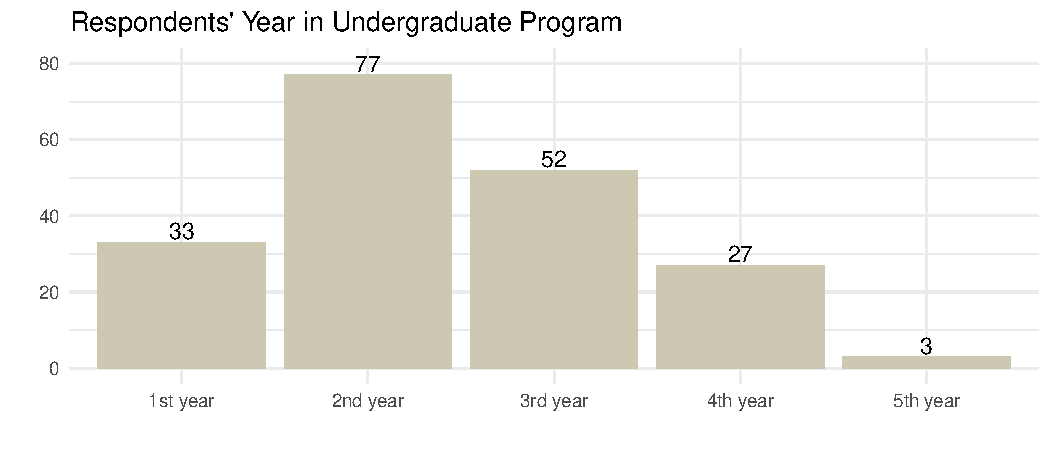
\includegraphics{GlobalHealthQuarto1-5_files/figure-pdf/unnamed-chunk-2-1.pdf}

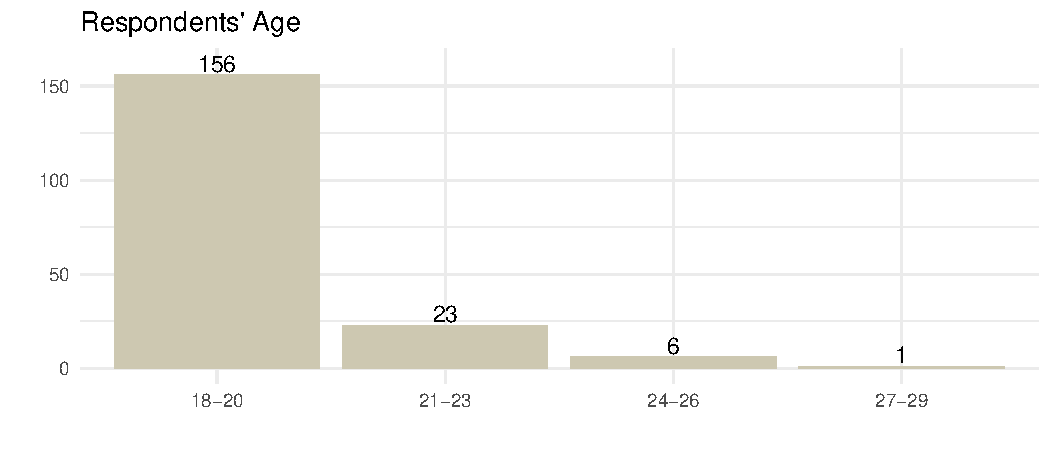
\includegraphics{GlobalHealthQuarto1-5_files/figure-pdf/unnamed-chunk-3-1.pdf}

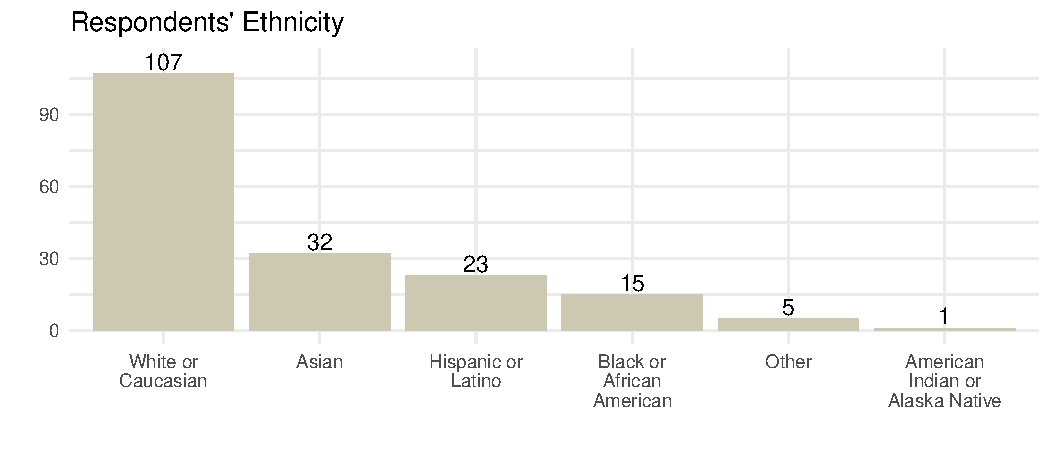
\includegraphics{GlobalHealthQuarto1-5_files/figure-pdf/unnamed-chunk-4-1.pdf}

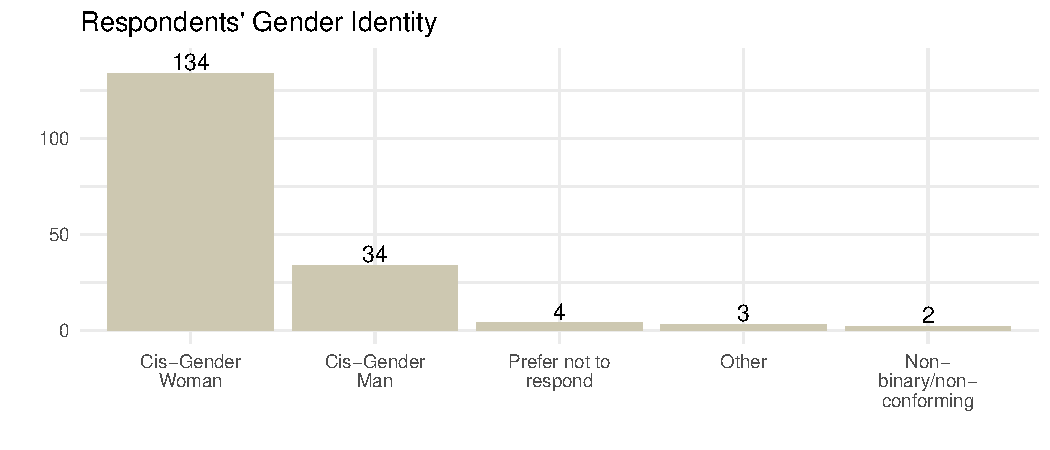
\includegraphics{GlobalHealthQuarto1-5_files/figure-pdf/unnamed-chunk-5-1.pdf}

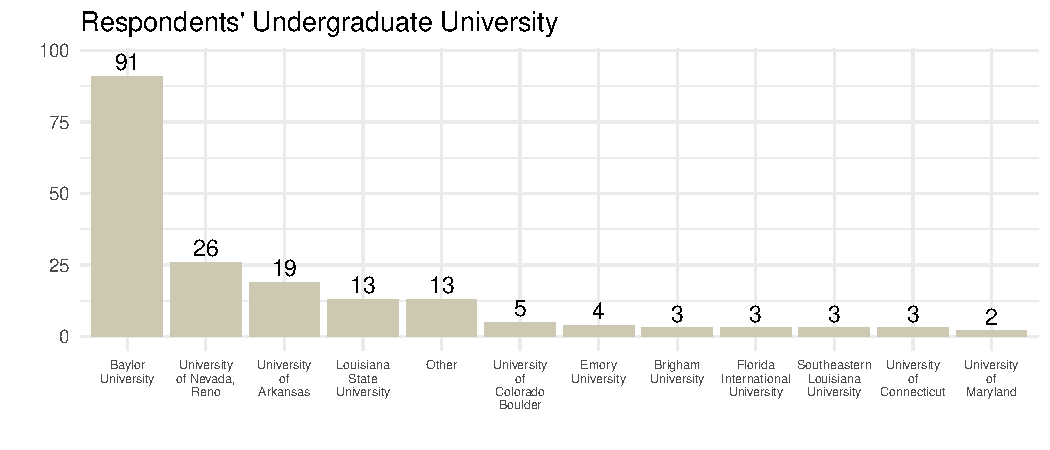
\includegraphics{GlobalHealthQuarto1-5_files/figure-pdf/unnamed-chunk-6-1.pdf}

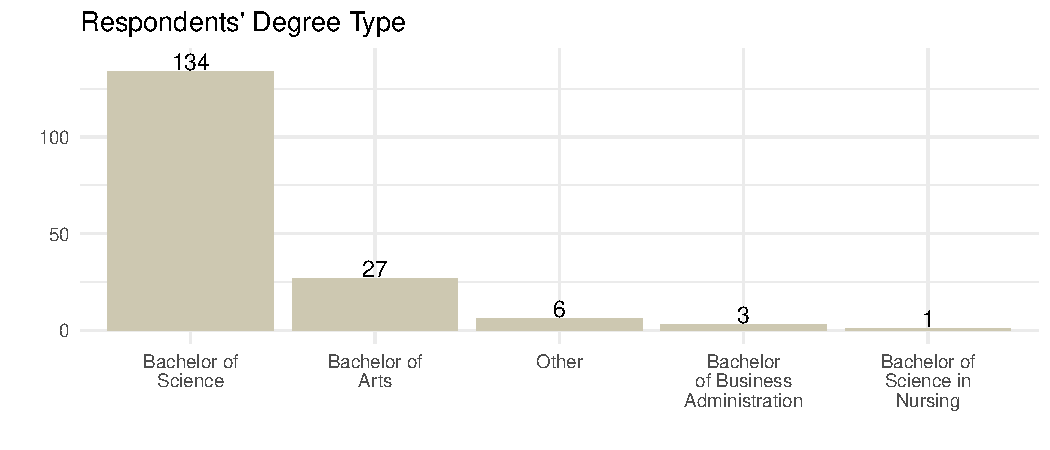
\includegraphics{GlobalHealthQuarto1-5_files/figure-pdf/unnamed-chunk-7-1.pdf}

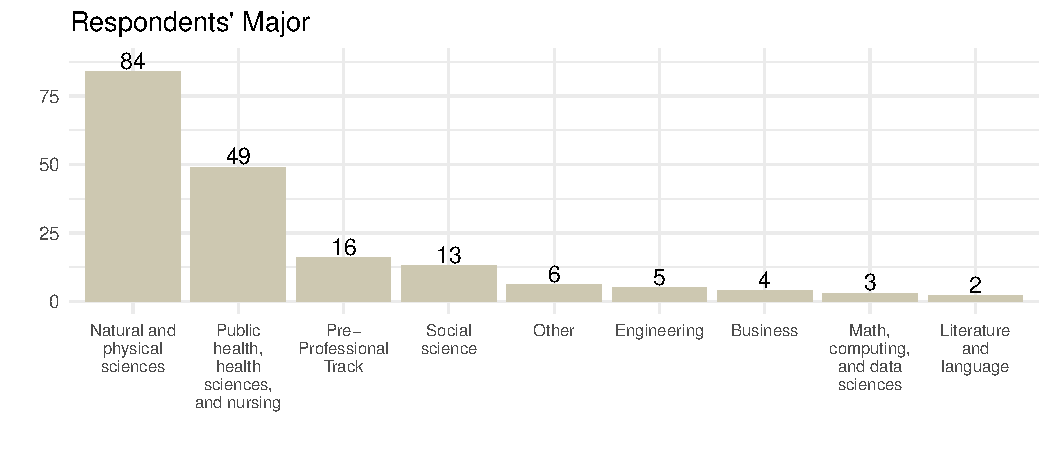
\includegraphics{GlobalHealthQuarto1-5_files/figure-pdf/unnamed-chunk-8-1.pdf}

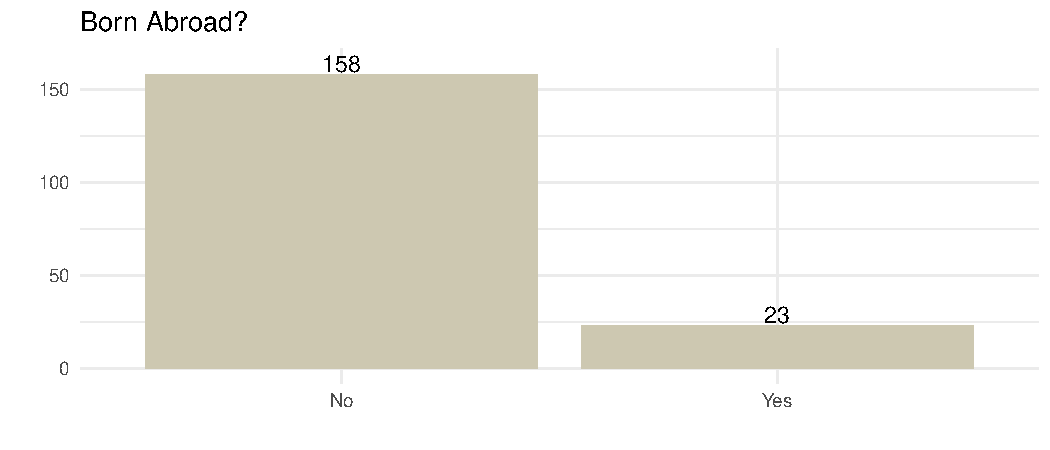
\includegraphics{GlobalHealthQuarto1-5_files/figure-pdf/unnamed-chunk-9-1.pdf}

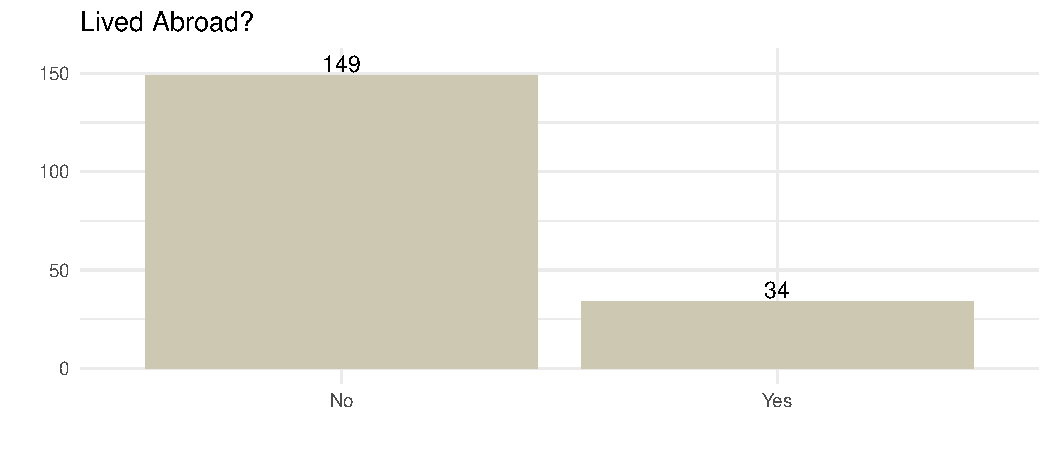
\includegraphics{GlobalHealthQuarto1-5_files/figure-pdf/unnamed-chunk-10-1.pdf}

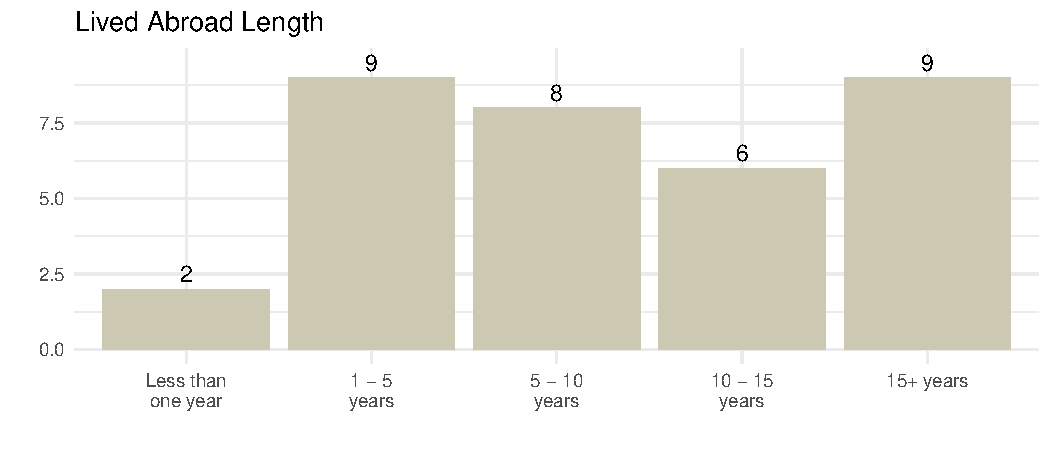
\includegraphics{GlobalHealthQuarto1-5_files/figure-pdf/unnamed-chunk-11-1.pdf}

\newpage

\hypertarget{how-do-pre-medical-students-perceive-a-career-in-global-health}{%
\subsection{2. How do pre-medical students perceive a career in global
health?}\label{how-do-pre-medical-students-perceive-a-career-in-global-health}}

A. Overall Responses to pursuing a career in Global Health.

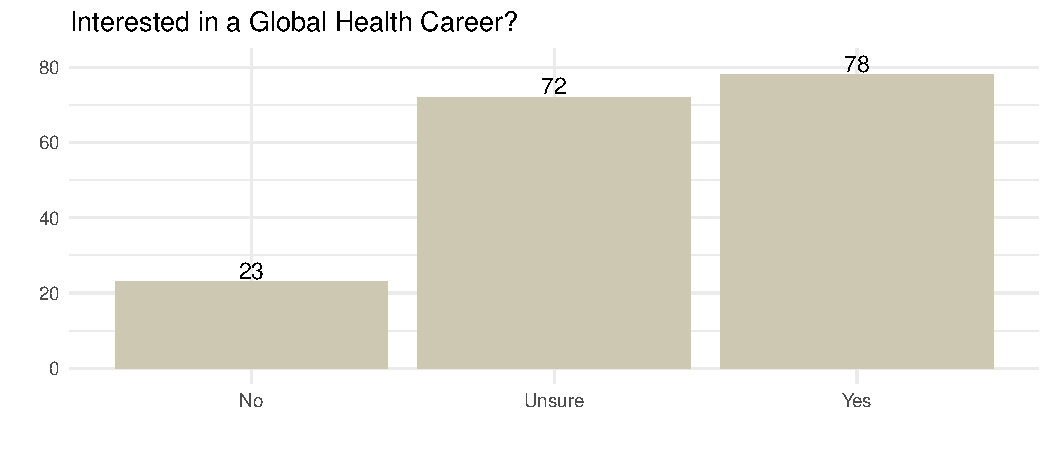
\includegraphics{GlobalHealthQuarto1-5_files/figure-pdf/unnamed-chunk-12-1.pdf}

\newpage

B. Pursuing a career in Global Health grouped by those who have lived
abroad.

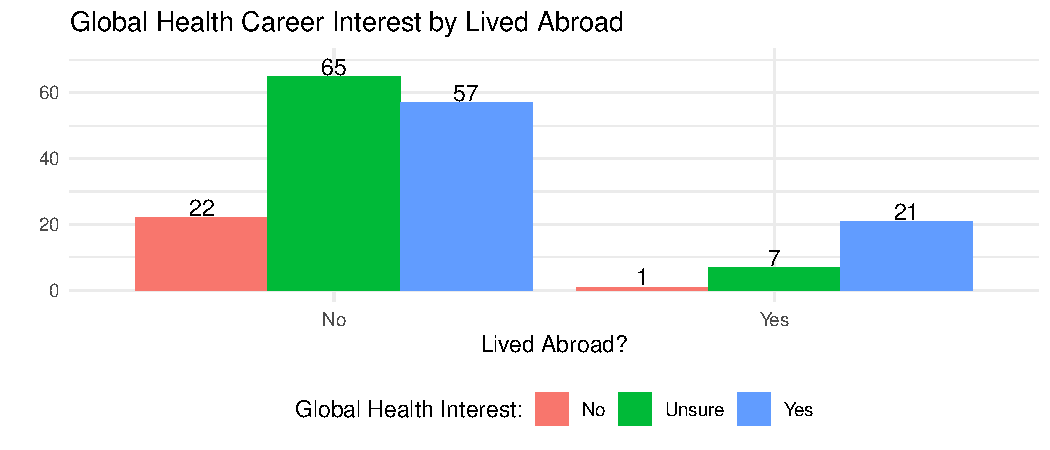
\includegraphics{GlobalHealthQuarto1-5_files/figure-pdf/unnamed-chunk-13-1.pdf}

\newpage

The following is a t-test measuring the difference in interest in a
Global Health Career in those who have lived outside the US and those
who have not. For this t-test I counted ``unsure'' responses as 1/2 a
``yes'' and 1/2 a ``no''. The results are significant. Those who have
lived outside the US demonstrate a higher interest in a Global Health
Career than those who have not lived outside the US.

\begin{verbatim}
# 
#   Welch Two Sample t-test
# 
# data:  df14ttest %>% filter(Q12 == "No") %>% select(Q14) and df14ttest %>% filter(Q12 == "Yes") %>% select(Q14)
# t = -3.8394, df = 49.077, p-value = 0.0003537
# alternative hypothesis: true difference in means is not equal to 0
# 95 percent confidence interval:
#  -0.3401720 -0.1064276
# sample estimates:
# mean of x mean of y 
# 0.6215278 0.8448276
\end{verbatim}

The following is also a t-test measuring the difference in interest in a
Global Health Career in those who have lived outside the US and those
who have not. For this t-test I removed ``unsure'' responses from the
data. Once again, the results are significant. Those who have lived
outside the US demonstrate a higher interest in a Global Health Career
than those who have not lived outside the US.

\begin{verbatim}
# 
#   Welch Two Sample t-test
# 
# data:  df14ttest %>% filter(Q12 == "No", Q14 != 0.5) %>% select(Q14) and df14ttest %>% filter(Q12 == "Yes", Q14 != 0.5) %>% select(Q14)
# t = -3.4202, df = 74.733, p-value = 0.001017
# alternative hypothesis: true difference in means is not equal to 0
# 95 percent confidence interval:
#  -0.36876272 -0.09729022
# sample estimates:
# mean of x mean of y 
# 0.7215190 0.9545455
\end{verbatim}

\newpage

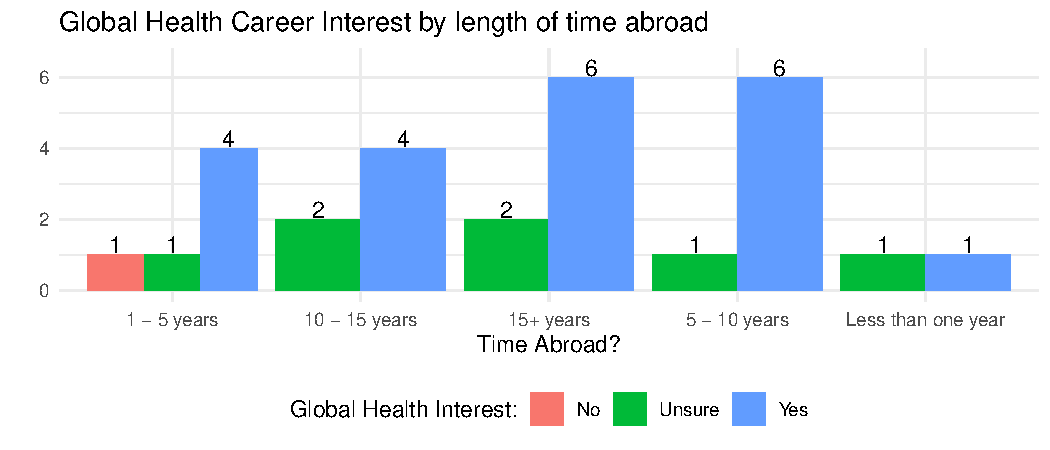
\includegraphics{GlobalHealthQuarto1-5_files/figure-pdf/unnamed-chunk-16-1.pdf}

\newpage

C. Pursuing a career in Global Health grouped by those who were born
abroad.

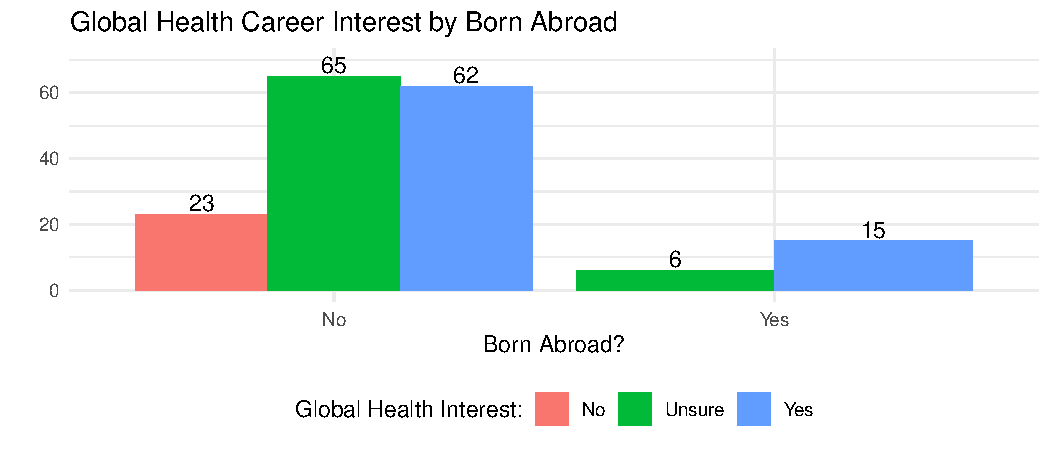
\includegraphics{GlobalHealthQuarto1-5_files/figure-pdf/unnamed-chunk-17-1.pdf}

\newpage

The following is a t-test measuring the difference in interest in a
Global Health Career in those who were born outside the US and those who
were not. For this t-test I counted ``unsure'' responses as 1/2 a
``yes'' and 1/2 a ``no''. The results are significant. Those who were
born outside the US demonstrate a higher interest in a Global Health
Career than those who were not born outside the US.

\begin{verbatim}
# 
#   Welch Two Sample t-test
# 
# data:  df14ttest %>% filter(Q10 == "No") %>% select(Q14) and df14ttest %>% filter(Q10 == "Yes") %>% select(Q14)
# t = -3.9021, df = 34.782, p-value = 0.000417
# alternative hypothesis: true difference in means is not equal to 0
# 95 percent confidence interval:
#  -0.3453416 -0.1089442
# sample estimates:
# mean of x mean of y 
# 0.6300000 0.8571429
\end{verbatim}

The following is a t-test measuring the difference in interest in a
Global Health Career in those who were born outside the US and those who
were not. For this t-test I removed ``unsure'' responses. The results
are significant. Those who were born outside the US demonstrate a higher
interest in a Global Health Career than those who were not born outside
the US.

\begin{verbatim}
# 
#   Welch Two Sample t-test
# 
# data:  df14ttest %>% filter(Q10 == "No", Q14 != 0.5) %>% select(Q14) and df14ttest %>% filter(Q10 == "Yes", Q14 != 0.5) %>% select(Q14)
# t = -5.5822, df = 84, p-value = 2.848e-07
# alternative hypothesis: true difference in means is not equal to 0
# 95 percent confidence interval:
#  -0.3669824 -0.1741941
# sample estimates:
# mean of x mean of y 
# 0.7294118 1.0000000
\end{verbatim}

\newpage

D. Pursuing a career in Global Health grouped by major.

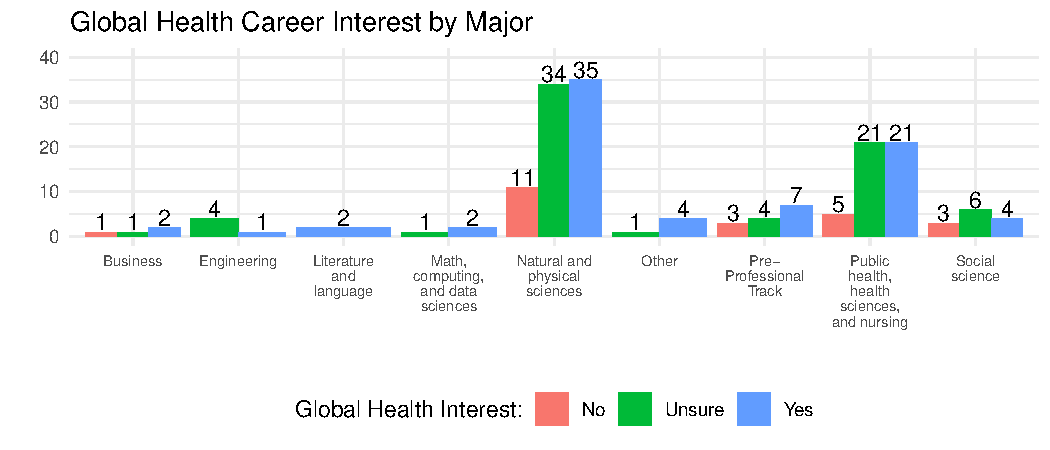
\includegraphics{GlobalHealthQuarto1-5_files/figure-pdf/unnamed-chunk-20-1.pdf}

\newpage

\hypertarget{which-aspects-of-the-global-health-field-interest-you-when-considering-your-medical-career}{%
\subsection{3. Which aspects of the global health field interest you
when considering your medical
career?}\label{which-aspects-of-the-global-health-field-interest-you-when-considering-your-medical-career}}

A. Total Results of Aspects of Global Health Field Considered

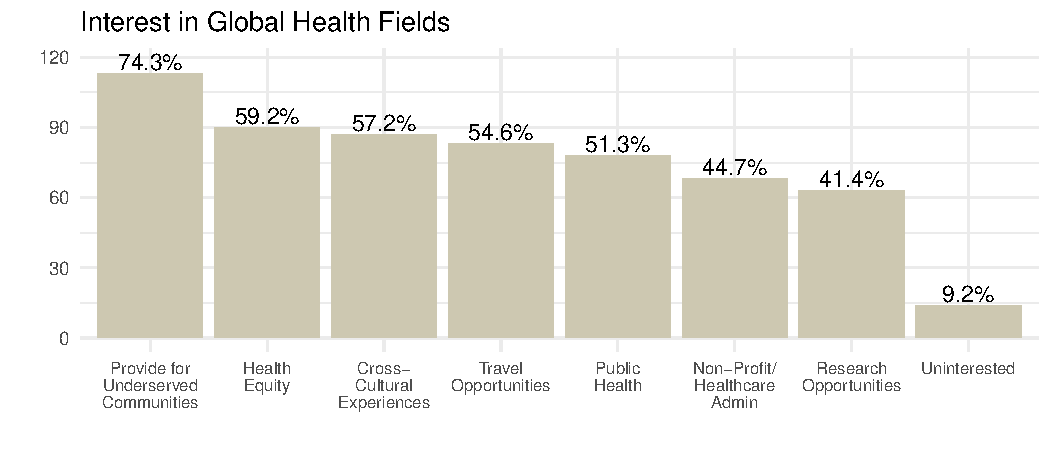
\includegraphics{GlobalHealthQuarto1-5_files/figure-pdf/unnamed-chunk-21-1.pdf}

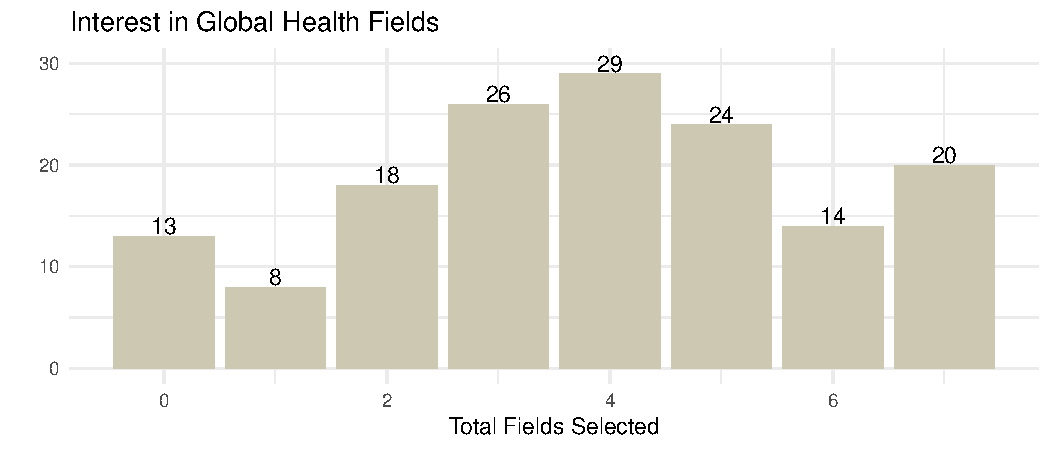
\includegraphics{GlobalHealthQuarto1-5_files/figure-pdf/unnamed-chunk-22-1.pdf}

\newpage

B. Results by Lived Outside the US

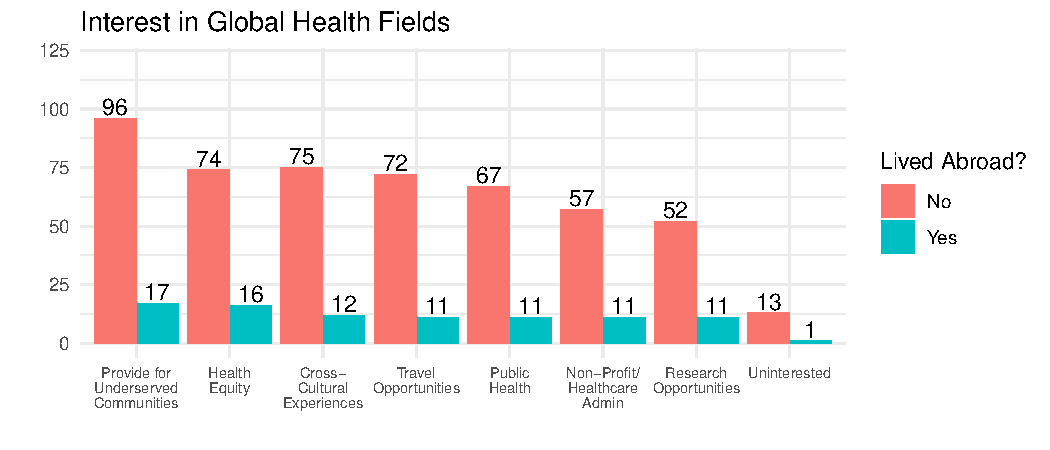
\includegraphics{GlobalHealthQuarto1-5_files/figure-pdf/unnamed-chunk-23-1.pdf}

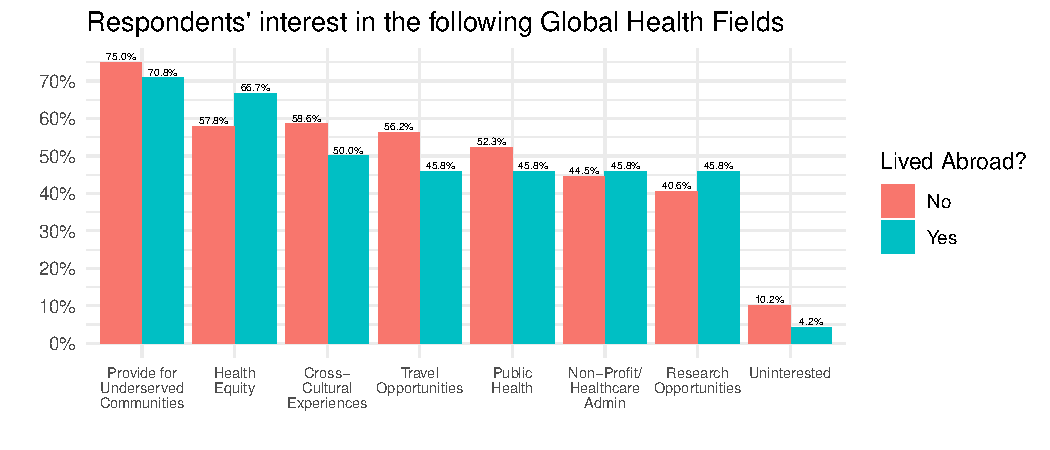
\includegraphics{GlobalHealthQuarto1-5_files/figure-pdf/unnamed-chunk-24-1.pdf}

\newpage

Below is a Chi Squared Test. This tests to see if the two distributions
of interest in the global health fields are distinct from one another.
The test cannot confirm that there is a distinction. In other words, the
difference in interest of the various global health fields of those who
lived abroad and those who did not live abroad is not significant.

\begin{verbatim}
# 
#   Pearson's Chi-squared test
# 
# data:  df15gLiveChi$Yes and df15gLiveChi$No
# X-squared = 32, df = 28, p-value = 0.2745
\end{verbatim}

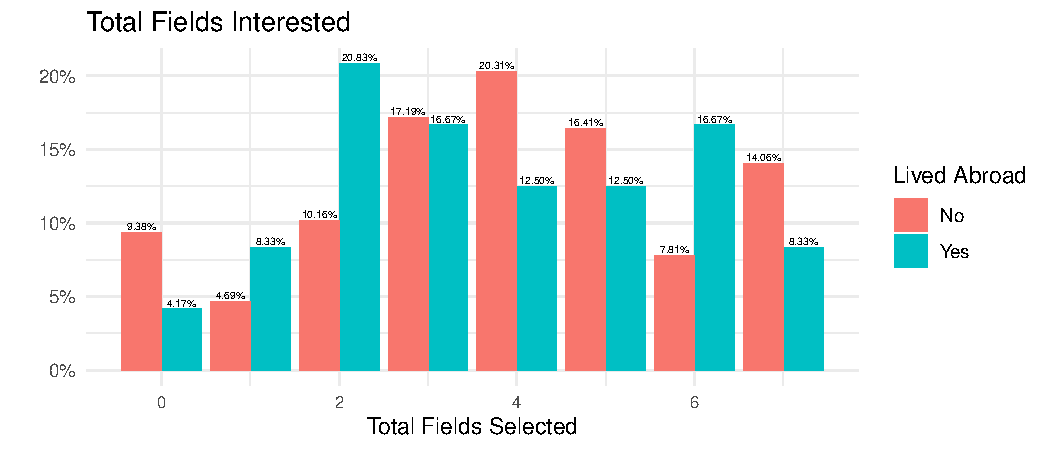
\includegraphics{GlobalHealthQuarto1-5_files/figure-pdf/unnamed-chunk-26-1.pdf}

Below is a second Chi Squared Test. This tests to see if the two
distributions are distinct from one another. The test cannot confirm
that there is a distinction. In other words, the difference between the
number of fields selected between those who lived abroad and did not
live abroad is insignificant.

\begin{verbatim}
# 
#   Pearson's Chi-squared test
# 
# data:  df15gLiveChiTotals$Yes and df15gLiveChiTotals$No
# X-squared = 32, df = 28, p-value = 0.2745
\end{verbatim}

\newpage

C. Results by born outside the US

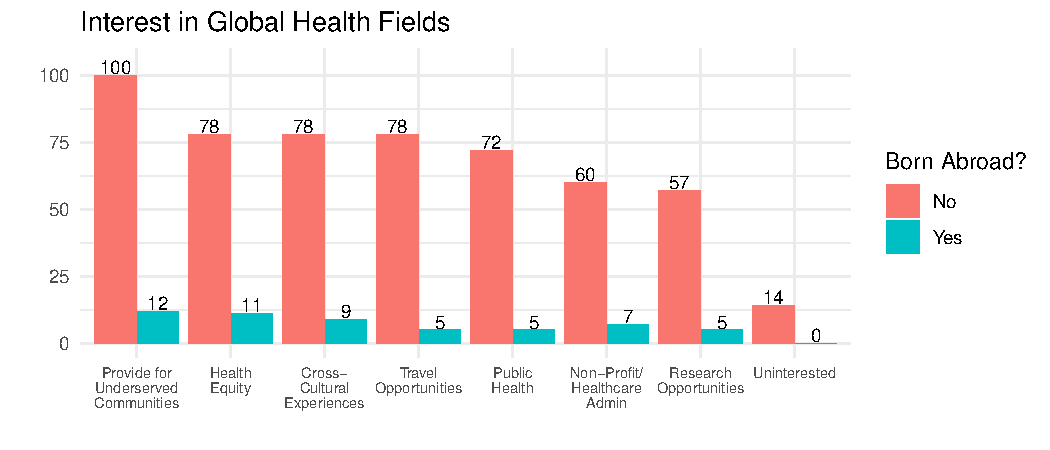
\includegraphics{GlobalHealthQuarto1-5_files/figure-pdf/unnamed-chunk-28-1.pdf}

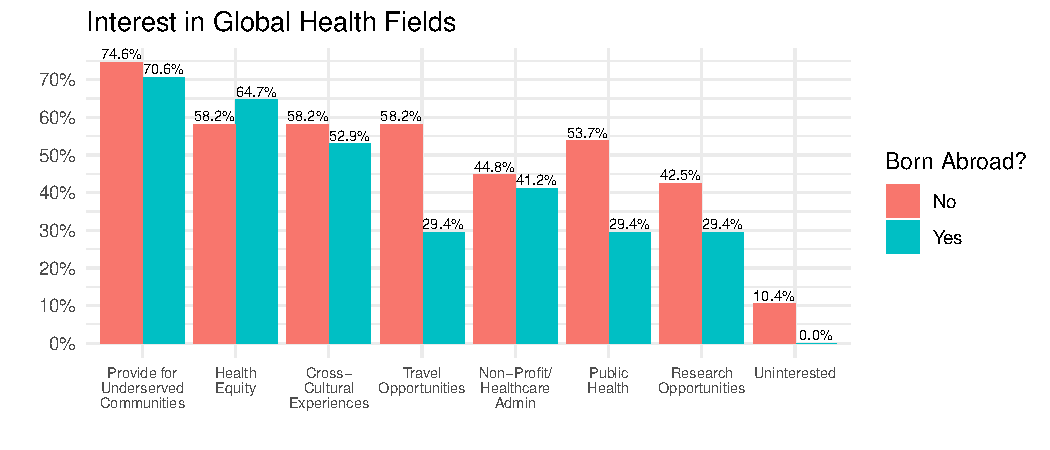
\includegraphics{GlobalHealthQuarto1-5_files/figure-pdf/unnamed-chunk-29-1.pdf}

\newpage

Below is a Chi Squared Test. This tests to see if the two distributions
of fields are distinct from one another. The test cannot confirm that
there is a distinction. In other words, the difference in interest of
the various global health fields of those who were born abroad and those
who were not born abroad is not significant.

\begin{verbatim}
# 
#   Pearson's Chi-squared test
# 
# data:  df15gBornChi$Yes and df15gBornChi$No
# X-squared = 27.556, df = 25, p-value = 0.3287
\end{verbatim}

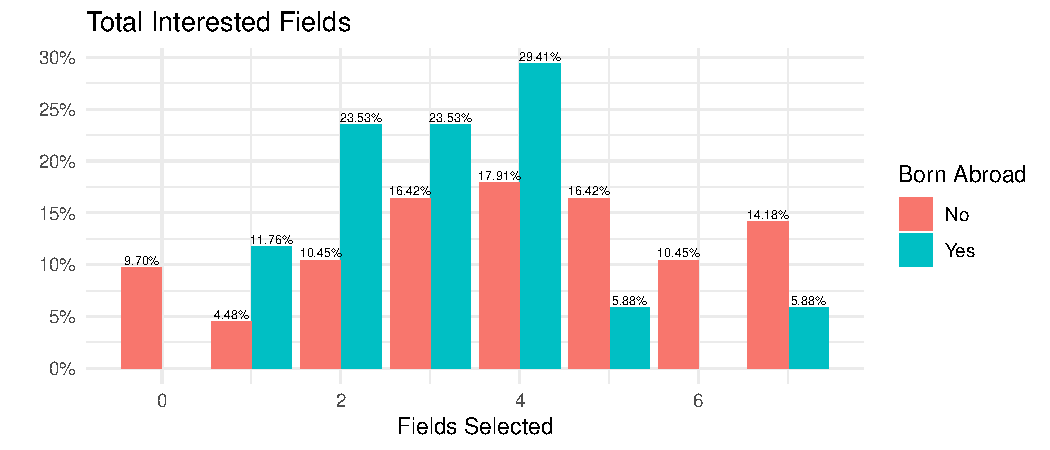
\includegraphics{GlobalHealthQuarto1-5_files/figure-pdf/unnamed-chunk-31-1.pdf}

Below is a Chi Squared Test. This tests to see if the two distributions
of the number of fields selected are distinct from one another. The test
cannot confirm that there is a distinction. In other words, the
difference in the total number of fields interested in by those who were
born abroad and those who were not born abroad is not significant.

\begin{verbatim}
# 
#   Pearson's Chi-squared test
# 
# data:  df15gBornChiTotals$Yes and df15gBornChiTotals$No
# X-squared = 18, df = 15, p-value = 0.2627
\end{verbatim}

\newpage

\hypertarget{in-your-opinion-in-addition-to-clinical-training-physicians-who-work-within-global-health-domestic-or-international-should-have-educational-training-in-which-three-academic-disciplines}{%
\subsection{4. In your opinion, in addition to clinical training,
physicians who work within global health (domestic or international)
should have educational training in which THREE academic
disciplines?}\label{in-your-opinion-in-addition-to-clinical-training-physicians-who-work-within-global-health-domestic-or-international-should-have-educational-training-in-which-three-academic-disciplines}}

A. Overall Results of educational training

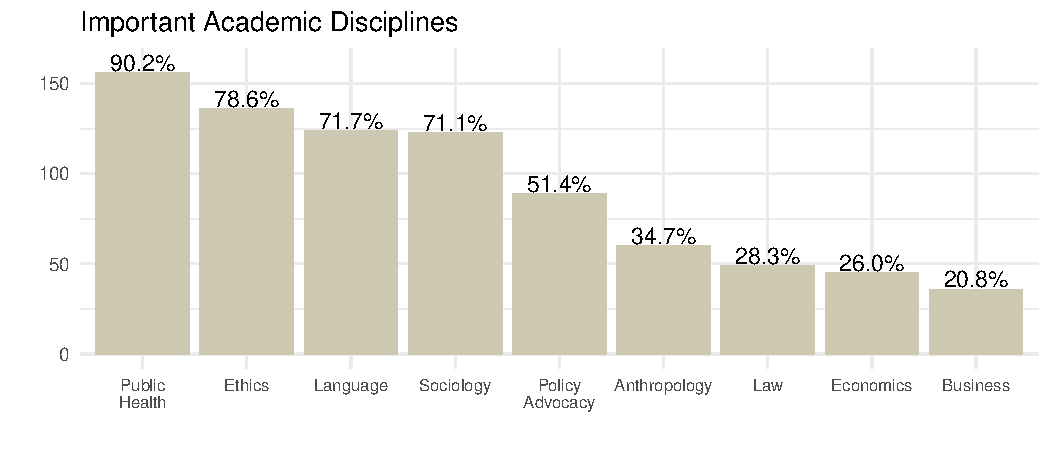
\includegraphics{GlobalHealthQuarto1-5_files/figure-pdf/unnamed-chunk-33-1.pdf}

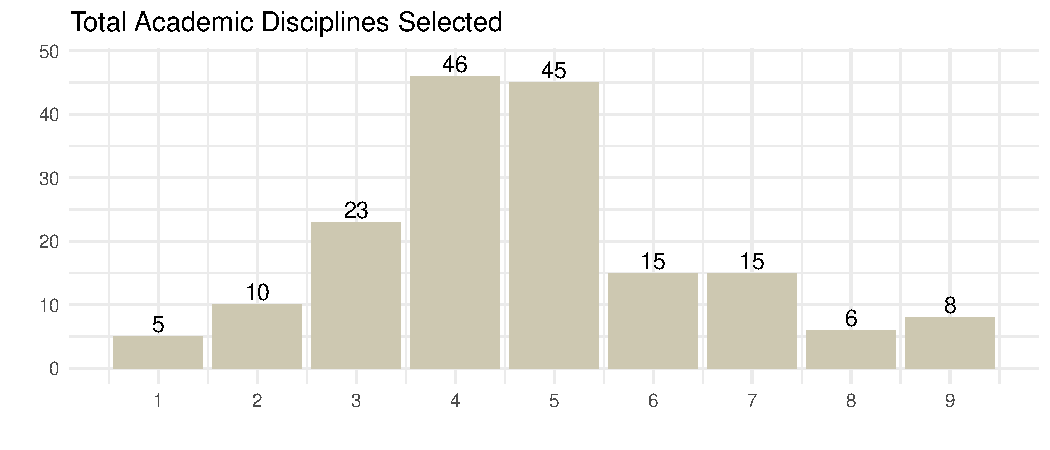
\includegraphics{GlobalHealthQuarto1-5_files/figure-pdf/unnamed-chunk-34-1.pdf}

\newpage

B. Relationship of preferred educational training with stated interest
in Global Health

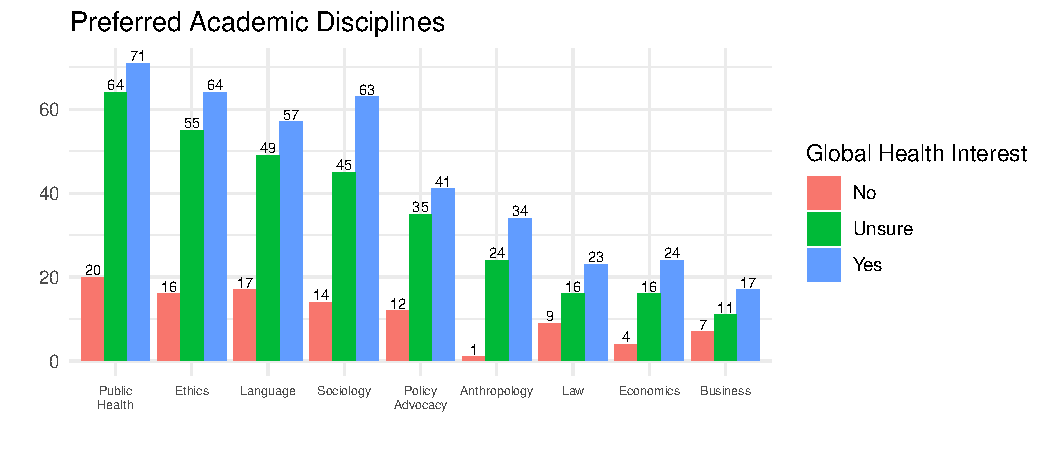
\includegraphics{GlobalHealthQuarto1-5_files/figure-pdf/unnamed-chunk-35-1.pdf}

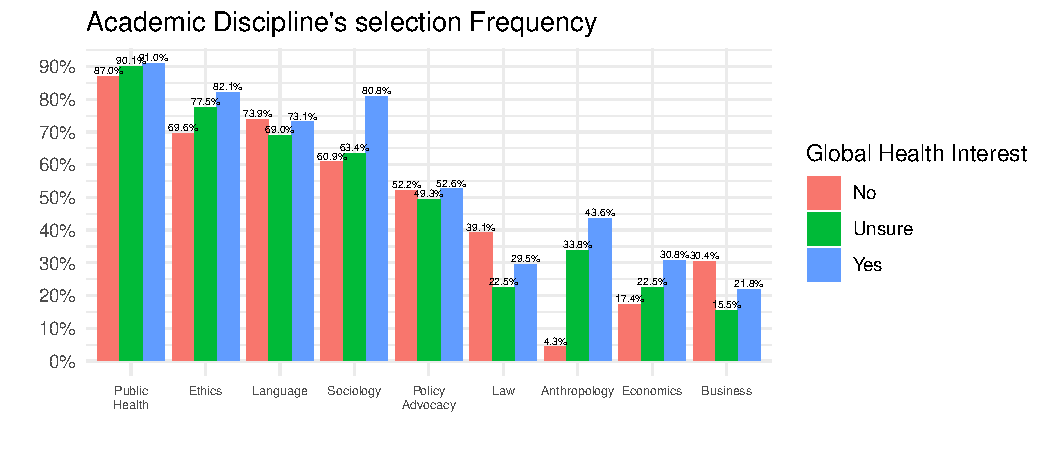
\includegraphics{GlobalHealthQuarto1-5_files/figure-pdf/unnamed-chunk-36-1.pdf}

\newpage

Below is a Chi Squared Test. This tests to see if the distribution of
the preference of academic disciplines preferred for global health is
distinct when separated by respondent's stated interest in Global
Health. The test cannot confirm that there is a distinction. In other
words, the difference in preference of the academic disciplines of those
who are interested in global health and who are not interested in global
health is not statistically significant.

\begin{verbatim}
# 
#   Pearson's Chi-squared test
# 
# data:  df16gIntChi$Yes and df16gIntChi$No
# X-squared = 72, df = 64, p-value = 0.2303
\end{verbatim}

\newpage

C. Correlation of preferred educational training with major

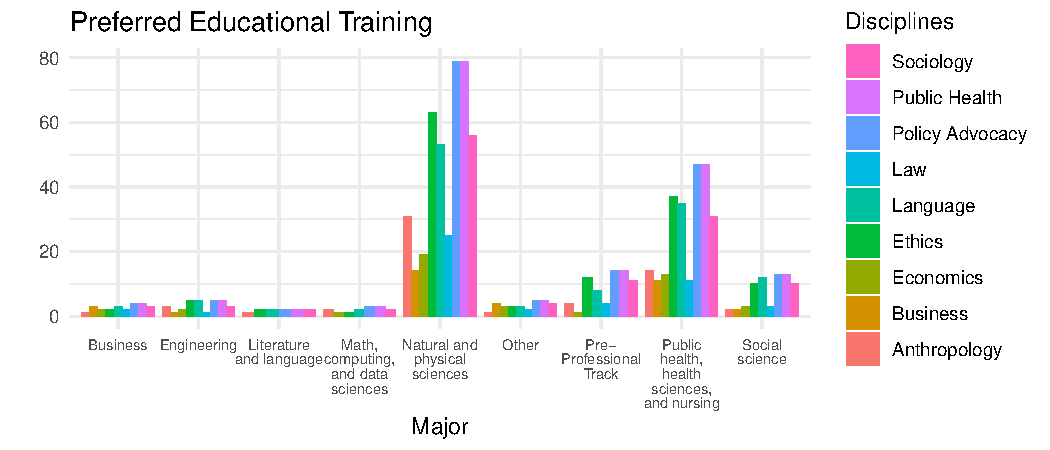
\includegraphics{GlobalHealthQuarto1-5_files/figure-pdf/unnamed-chunk-38-1.pdf}

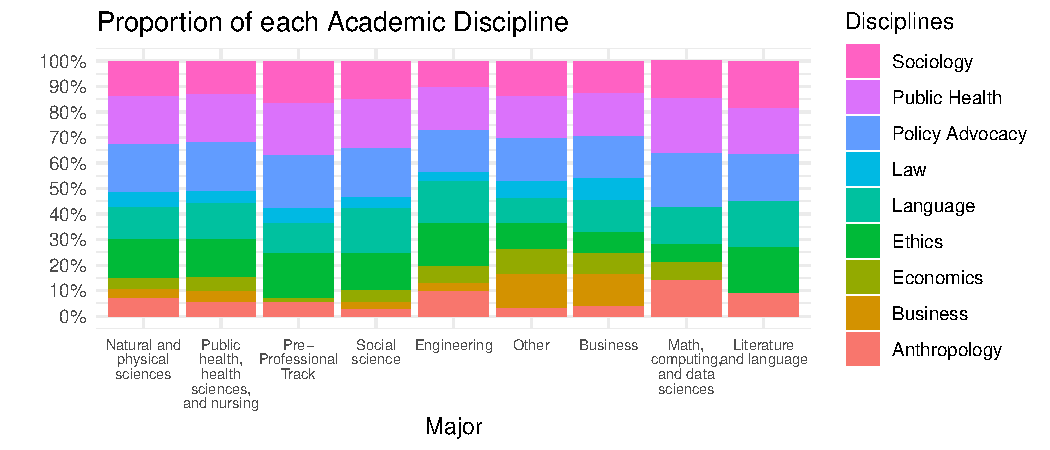
\includegraphics{GlobalHealthQuarto1-5_files/figure-pdf/unnamed-chunk-39-1.pdf}

\newpage

\hypertarget{should-all-pre-medical-students-take-at-least-one-global-health-focused-class-before-entering-medical-school}{%
\subsection{5. Should all pre-medical students take at least one global
health-focused class before entering medical
school?}\label{should-all-pre-medical-students-take-at-least-one-global-health-focused-class-before-entering-medical-school}}

A. Overall Results of Global Health Class Requirement

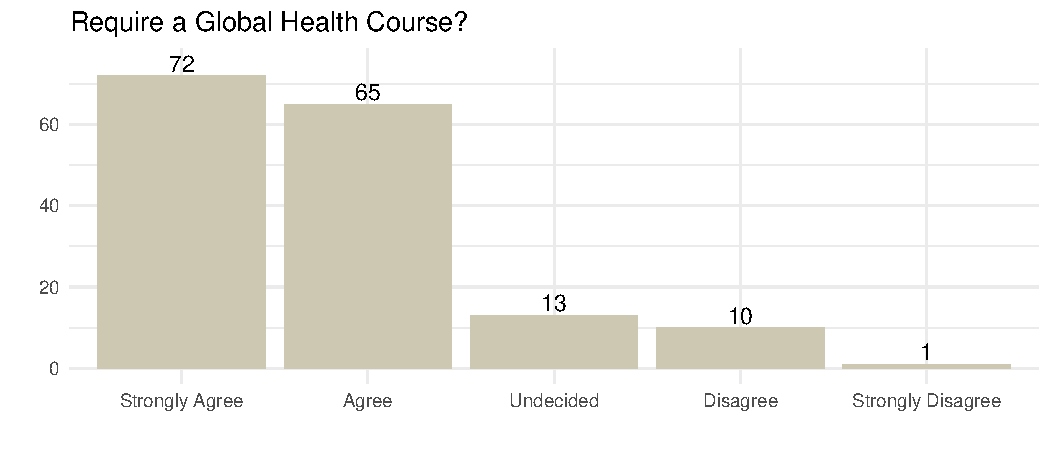
\includegraphics{GlobalHealthQuarto1-5_files/figure-pdf/unnamed-chunk-40-1.pdf}

\newpage

B. Global Health Class Requirement by Global Health Career Interest

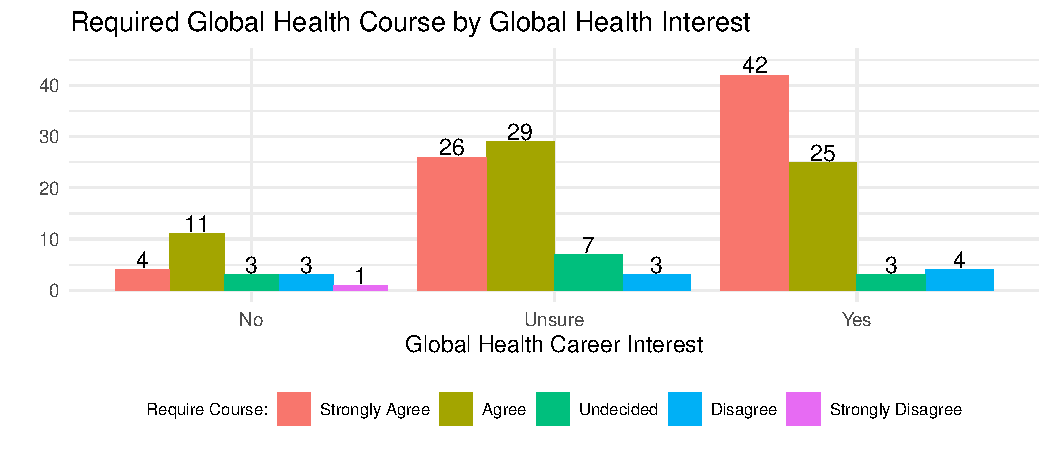
\includegraphics{GlobalHealthQuarto1-5_files/figure-pdf/unnamed-chunk-41-1.pdf}

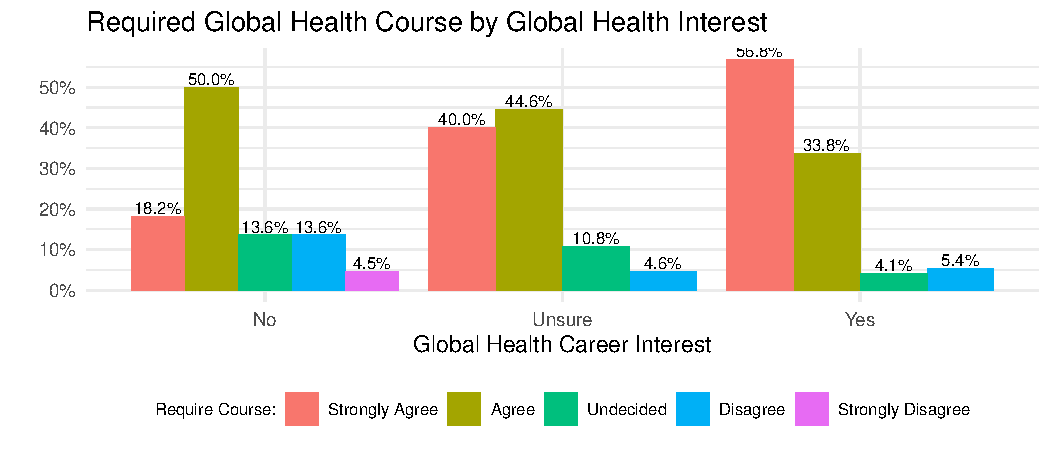
\includegraphics{GlobalHealthQuarto1-5_files/figure-pdf/unnamed-chunk-42-1.pdf}

\newpage

C. Global Health Class Requirement by Living Abroad

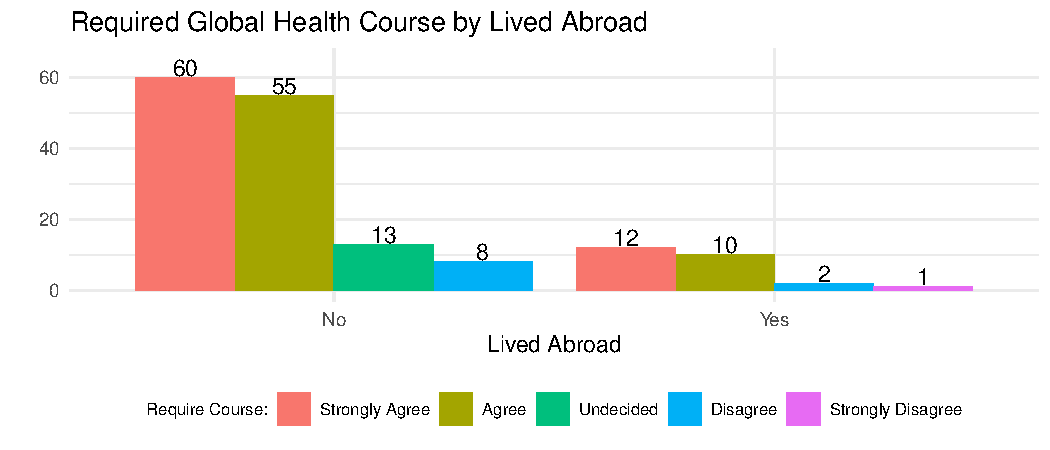
\includegraphics{GlobalHealthQuarto1-5_files/figure-pdf/unnamed-chunk-43-1.pdf}

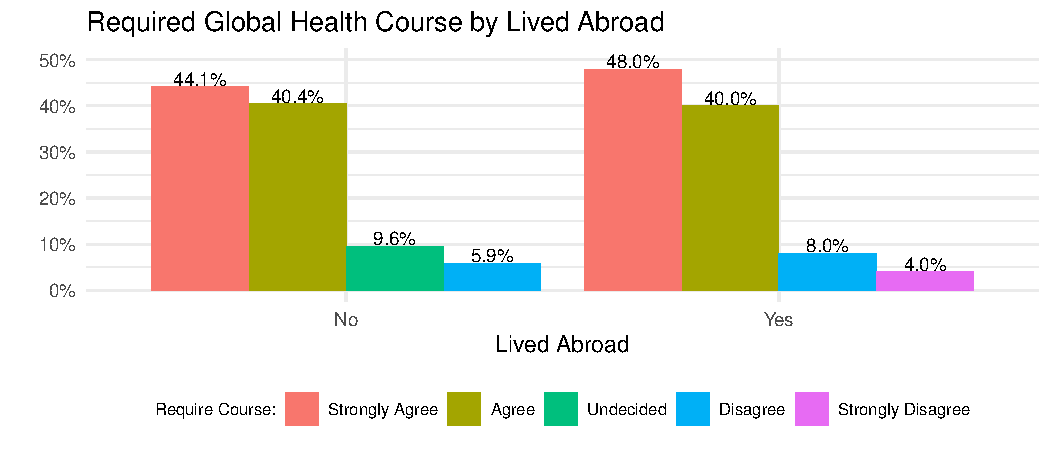
\includegraphics{GlobalHealthQuarto1-5_files/figure-pdf/unnamed-chunk-44-1.pdf}

\newpage

D. Global Health Class Requirement by Major

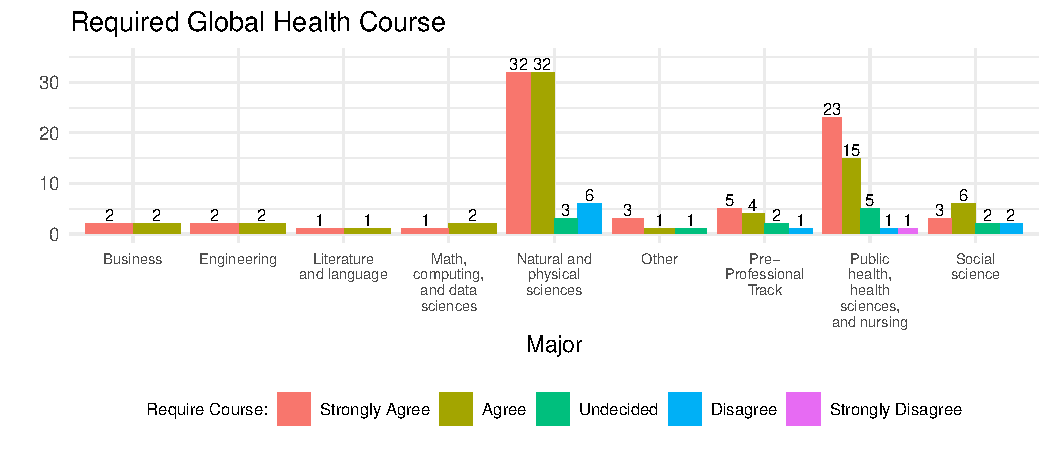
\includegraphics{GlobalHealthQuarto1-5_files/figure-pdf/unnamed-chunk-45-1.pdf}

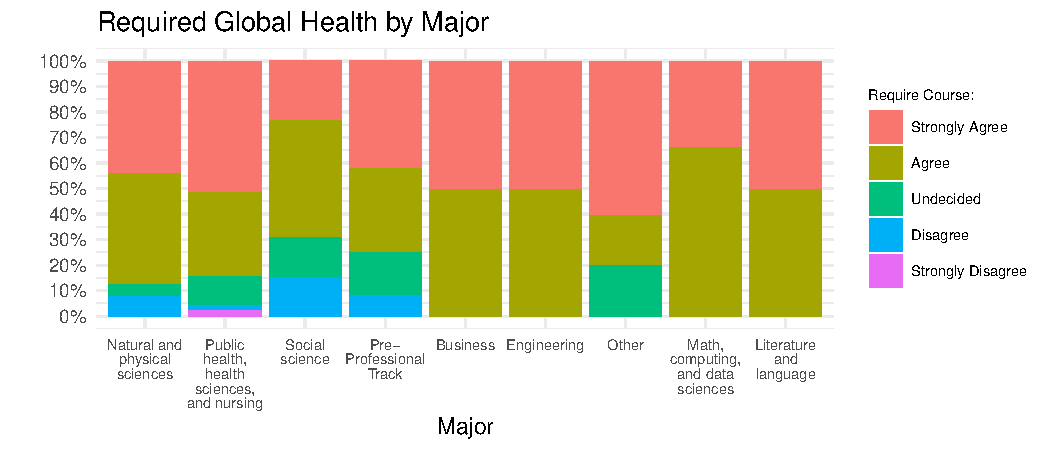
\includegraphics{GlobalHealthQuarto1-5_files/figure-pdf/unnamed-chunk-46-1.pdf}



\end{document}
